\documentclass{beamer}
\usepackage[british]{babel}
\usepackage{graphicx,hyperref,ru,url}
\usepackage[utf8x]{inputenc}
%https://www.cs.usfca.edu/~galles/visualization/Algorithms.html
\title[Universidade Federal de Alagoas]{
  Red-Black Tree}

\subtitle{Balanced Binary Search Tree}

\author[Data Structure]{
  Hiago Lopes Cavalcante\\João Pedro Brito Tomé\\John Davi Dutra Canuto Pires\\Luana Júlia Nunes Ferreira\\Ruan Heleno Correa da Silva\medskip}
  
\institute[Instituto de Computação]{
  Universidade Federal de Alagoas\\ Instituto de Computação}

\date[Red-Black Tree]{25 de março de 2019}

\begin{document}

\begin{frame}
  \titlepage
\end{frame}

\begin{frame}
    \frametitle{Outline}
    \tableofcontents
\end{frame}

\section{Motivation}

\subsection{Binary Search Tree}

\begin{frame}{Previous in BST classes...}
Let's consider adding theses numbers: 9, 8, 8, 0, 2, 0, 4, 4, 3. %https://www.cs.usfca.edu/~galles/visualization/BST.html
\begin{center}
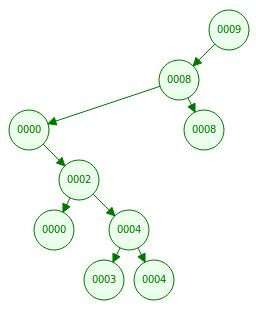
\includegraphics[scale=0.6]{bst.jpeg}
\end{center}
\end{frame}

\begin{frame}{Troubles start to show up...}
\justifying
What if we add the same numbers in descending order?\\ \\
\begin{columns}
\begin{column}{0.5\textwidth}
   \begin{block}{Low efficiency:}\end{block}
   \begin{itemize}
       \item Search;
       \item Insert;
       \item Delete;
   \end{itemize}
   \begin{block}{It runs $O(n)$!}\end{block}
\end{column}
\begin{column}{0.5\textwidth}
    \begin{center}
     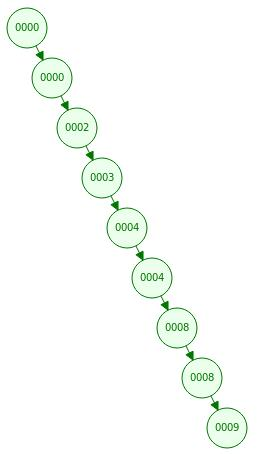
\includegraphics[width=0.6\textwidth]{bst_order.jpeg}
     \end{center}
\end{column}
\end{columns}
%https://www.cs.usfca.edu/~galles/visualization/BST.html
%http://inst.eecs.berkeley.edu/~cs61b/fa17/materials/demos/ll-red-black-demo.html
\end{frame}

\subsection{AVL Tree}

\begin{frame}{AVL tree}

\begin{columns}
\begin{column}{0.5\textwidth}
   \begin{block}{What do we need? BALANCE!\\And here it comes: AVL Tree!}\end{block}
 \begin{itemize}
    \item 4 kinds of rotations (L-L, R-R, R-L, L-R);
    \item Balance Factor: 0, -1 or 1;
    \item Searching in AVL is close to O(log n).
\end{itemize}
\end{column}
\begin{column}{0.5\textwidth}
    \begin{center}
     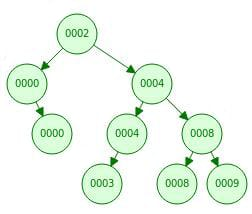
\includegraphics[width=0.9\textwidth]{avl.jpeg}
     \end{center}
\end{column}
\end{columns}
\end{frame}

\begin{frame}{But...}
\centering\color{red}{\Huge AVL needs too many rotations!!!}
\end{frame}

\section{The Red-Black Tree}
\subsection{Definition}

\begin{frame}{The Red-Black Tree}
    \begin{center}
     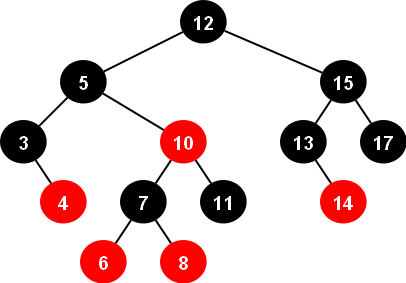
\includegraphics[width=0.8\textwidth]{redblacktree.png}
     \end{center}
\end{frame}

\begin{frame}{Definition}
\begin{itemize}
    \item \Large A Binary Search Tree with an extra bit to hold the color:
\end{itemize}
\centering\color{red}{\textbf{RED = 1}}\\\color{black}{\textbf{BLACK = 0}}
\begin{itemize}
    \item \Large It ensures the tree remains balanced.
\end{itemize}
\end{frame}

\subsection{Red-black Structure}
\begin{frame}{Red-Black Structure}
\begin{columns}
\begin{column}{0.5\textwidth}
   \justifying
   \begin{algorithm}
   \SetAlgoLined
   {
       
        struct redblack\\
        \{\\
            \STATE  \ \ \ \ int item;\\
            \STATE  \ \ \ \ int color;\\
            \STATE  \ \ \ \ redblack *left;\\
            \STATE  \ \ \ \ redblack *right;\\
        \}\\
   }
\end{algorithm} %Struct 
\end{column}
\begin{column}{0.5\textwidth}
    \begin{center}
     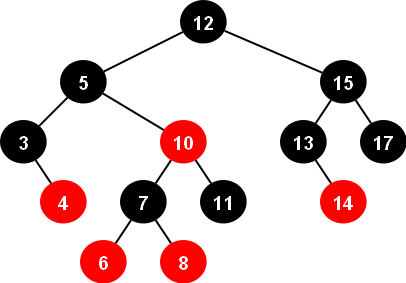
\includegraphics[width=1.0\textwidth]{redblacktree.png}
     \end{center}
\end{column}
\end{columns}
\end{frame}

\subsection{Advantages of Red-Black}
\begin{frame}{Advantages of Red-Black}
\begin{enumerate}
    \item Rotations run in \textcolor{red}{O(1)};
    \item Searching, insertion and deletion run in \textcolor{red}{O(log n)};
    \item In remotion, the RB tree rotates once (with single or double rotation), while the AVL tree can rotate \textcolor{red}{log n} times; 
\end{enumerate}
\end{frame}

\subsection{Properties}
\begin{frame}{Properties}
\begin{itemize}
    \item Every node is either red or black;
    \item The root and leaves \textbf{(NIL’s)} are black;
    \item If a node is \textcolor{red}{red}, then its parent is black;
    \item For each node, every path from the node to the descendant leaves contains the same number of \textbf{BLACK} nodes.
\end{itemize}
\end{frame}

\begin{frame}{Properties}
\begin{itemize}
    \item There can't be two consecutive red nodes in a path from the root to a sub-tree; \item The properties are checked every time a operation is done in the RB tree;
    \item In case some property is not satisfied, rotations and color flips are done.
\end{itemize}
\end{frame}

\subsection{Black Height}
\begin{frame}{Black Height}
It is the number of \textbf{BLACK} nodes found until any descendant node.
A red-black tree with $n$ keys has height:
\begin{equation*}
\color{red}h ≤ 2log(n + 1)   
\end{equation*}
\begin {center}
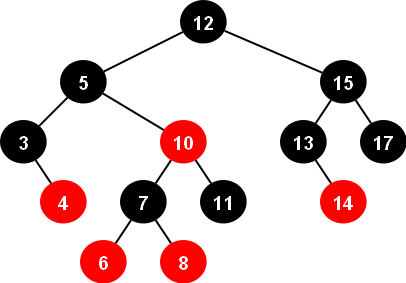
\includegraphics[scale=0.3]{redblacktree.png}
\end {center}
\end{frame}

\subsection{Insertion}
\begin{frame}{Color Flip}

\begin{left}
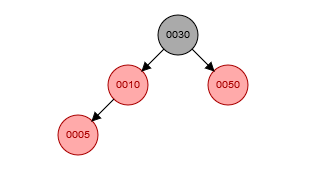
\includegraphics[scale=0.6]{RECOLOR1.png}
\end{left}
\begin{right}
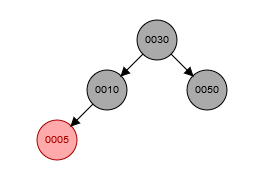
\includegraphics[scale=0.7]{RECOLOR2.png}
\end{right}

\end{frame}

\begin{frame}{Right Rotation}
\begin{left}
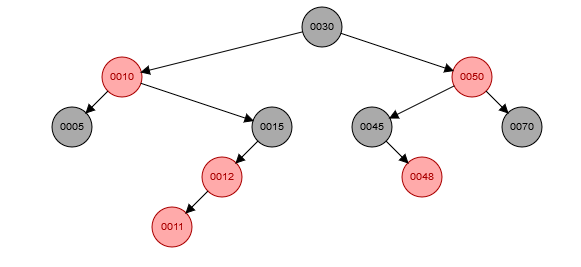
\includegraphics[scale=0.5]{LL1.png}
\end{left}
\begin{right}
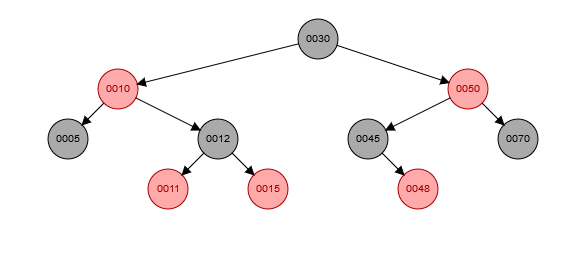
\includegraphics[scale=0.5]{LL2.png}
\end{right}
\end{frame}

\begin{frame}{Left Rotation}
\begin{left}
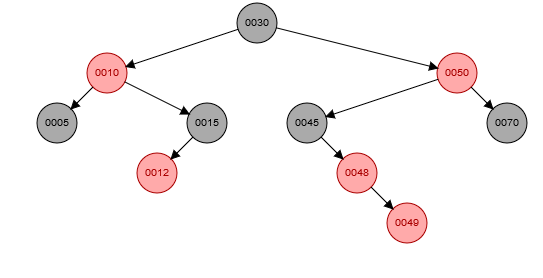
\includegraphics[scale=0.5]{RR1.png}
\end{left}
\begin{right}
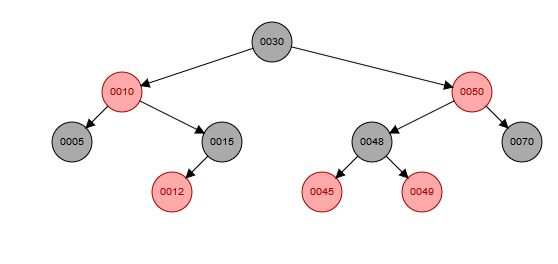
\includegraphics[scale=0.5]{RR2.png}
\end{right}
\end{frame}

\section{Abstract Data Type}
\begin{frame}{Abstract Data Type}
btree* create\_empty\_btree();\\
btree* rotate\_left(btree *bt);\\
btree* rotate\_right(btree *bt);\\
btree* move\_left\_red(btree *bt);\\
btree* move\_right\_red(btree *bt);\\
btree* balance\_factor(btree *bt);\\
btree* add\_bt(btree *bt, int value);\\
btree* add\_arv(btree *bt, int value);\\
btree* remove\_bt(btree *bt, int value);\\
btree* remove\_arv(btree *bt, int value);\\
int search(btree *bt, int value, int *flag);\\
int color(btree *bt);\\
void print\_pre\_order(btree *bt);\\
void color\_swap(btree *bt);
\end{frame}

\section{Functions and Implementation}
\subsection{Add}
\begin{frame}{Add}
\tiny{btree* add\_bt(btree *bt, int value)\\
\{\\
    if(bt == NULL)\\
    \{\\
        btree *new\_btree = (btree*) malloc ( sizeof(btree) );\\
        if(new\_btree == NULL) return NULL;\\
        new\_btree \rightarrow item = value;\\
        new\_btree \rightarrow color = RED;\\
        new\_btree \rightarrow left = NULL;\\
        new\_btree \rightarrow right = NULL;\\
        return new\_btree;\\
    \}\\
    if(value != bt \rightarrow item)\\
    \{\\
        if(value $<$ bt \rightarrow item)\quad bt->left = add\_bt(bt \rightarrow left, value);\\
        else if(value $>$ bt \rightarrow item)\quad bt \rightarrow right = add\_bt(bt \rightarrow right, value);\\
    \}\\
    if(color(bt \rightarrow right) == RED\quad \&\&\quad color(bt \rightarrow left) == BLACK)\quad bt = rotate\_left(bt);\\
    if(color(bt \rightarrow left) == RED\quad \&\&\quad color(bt \rightarrow left \rightarrow left) == RED) \quad bt = rotate\_right(bt);\\
    if(color(bt \rightarrow left) == RED\quad \&\&\quad color(bt \rightarrow right) == RED)\\ color\_swap(bt);\\
    return bt;\\
\}}
\end{frame}

\subsection{Balance Factor}
\begin{frame}{Balance Factor}
btree* balance\_factor(btree *bt);\\
\{\\
    if(color(bt \rightarrow right) == RED) \quad bt = rotate\_left(bt);\\
    if(bt \rightarrow left != NULL \quad\&\&\quad color(bt \rightarrow right) == RED \quad\&\&\quad \\ color(bt \rightarrow left \rightarrow left) == RED) \quad bt = rotate\_right(bt);\\
    if(color(bt \rightarrow left) == RED \quad\&\&\quad color(bt \rightarrow right) == RED) \quad color\_swap(bt);\\
    return bt;\\
\}    
\end{frame}

\subsection{Rotations}
\begin{frame}{Rotate Left and Rotate Right}
\begin{columns}
\begin{column}{0.5\textwidth}
   \justifying
   btree* rotate\_left(btree *bt)\\
\{\\
    btree *aux = bt \rightarrow right;\\
    bt \rightarrow right = aux \rightarrow left;\\
    aux \rightarrow left = bt;\\
    aux \rightarrow color = bt \rightarrow color;\\
    bt \rightarrow color = RED;\\
    return aux;\\
\}
\end{column}
\begin{column}{0.5\textwidth}
    \justifying
    btree* rotate\_right(btree *bt)\\
\{\\
    btree *aux = bt \rightarrow left;\\
    bt \rightarrow left = aux \rightarrow right;\\
    aux \rightarrow right = bt;\\
    aux \rightarrow color = bt \rightarrow color;\\
    bt \rightarrow color = RED;\\
    return aux;\\
\}
\end{column}
\end{columns}
\end{frame}

\begin{frame}{Move Left Red and Move Right Red}
\begin{columns}
\begin{column}{0.5\textwidth}
   \justifying
   btree* move\_left\_red(btree *bt)\\
\{\\
    color\_swap(bt);\\
    if(color(bt \rightarrow right \rightarrow left) == RED)\\
    \{\\
        bt \rightarrow right = rotate\_right(bt \rightarrow right);\\
        bt = rotate\_left(bt);\\
        color\_swap(bt);\\
    \}\\ return bt;\\
\}
\end{column}
\begin{column}{0.5\textwidth}
    \justifying
    btree* move\_right\_red(btree *bt)\\
\{\\
    color\_swap(bt);\\
    if(color(bt \rightarrow left \rightarrow left) == RED)\\
    \{\\
        bt = rotate\_right(bt);\\
        color\_swap(bt);\\
    \}\\ return bt;\\
\}
\end{column}
\end{columns}
\end{frame}

\subsection{Remove and Search}
\begin{frame}{Remove}
\scriptsize{btree* remove\_bt(btree *bt, int value)\\
\{\\
        if(value $<$ bt \rightarrow item)\\
        \{\\
            if(color(bt \rightarrow left) == BLACK \quad\&\&\quad color(bt \rightarrow left \rightarrow left) == BLACK) \quad bt = move\_left\_RED(bt);\\
            bt \rightarrow left = remove\_bt(bt \rightarrow left, value);
        \}\\
        else
        \{\\
            if(color(bt \rightarrow left) == RED) \quad bt = rotate\_right(bt);\\
            if(value == bt \rightarrow item \quad\&\&\quad bt \rightarrow right == NULL) \quad \{free(bt); return NULL;\}\\
            if(color(bt \rightarrow right) == BLACK \quad\&\&\quad color(bt \rightarrow right \rightarrow left) == BLACK) \quad bt = move\_right\_RED(bt);
            if(value == bt \rightarrow item)\\
            \{\\
                btree *aux = minor\_search(bt \rightarrow right);\\
                bt \rightarrow item = aux \rightarrow item;\\
                bt \rightarrow right = minor\_remove(bt \rightarrow right);\\
            \} \quad else bt \rightarrow right = remove\_bt(bt \rightarrow right, value);\\
        \}\\
        return balance\_factor(bt);\\
\}}
\end{frame}

\begin{frame}{Search}
int search(btree *bt, int value, int *flag)\\
\{\\
    if(bt != NULL)\\
    \{\\
        if(bt \rightarrow item == value) \quad *flag = 1;\\
        search(bt \rightarrow left, value, flag);\\
        search(bt \rightarrow right, value, flag);\\
    \}\\
    return *flag;\\
\}    
\end{frame}

\begin{frame}{Animation}
\begin{center}
    bit.ly/gifredblack\\
    imgur.com/vV1RDz5
\end{center}
\end{frame}

\begin{frame}{Conclusion}
Red-Black Trees can be very useful!
\begin{enumerate}
    \item Running time: \textcolor{red}{O(log n)};
    \item Rotations: \textcolor{red}{O(1)};
\end{enumerate}    
\end{frame}

\begin{frame}{References}
\begin{itemize}
\item \small{E.Demaine, \textbf{"Introduction to algorithms"}, Lecture 10, Massachusetts Institute of technology Open Course, 2015;}
\item \small{S. W. Song, \textbf{"Árvore Rubro-Negra"}, Estruturas de Dados, Universidade de São Paulo - IME/USP, 2008;}
\item \small{T. H. Cormen, C. E. Leiserson, R. L. Rivest, C. Stein, \textbf{"Introduction to Algorithms"}, 2º edition, MIT Press \& McGraw-Hill, 2001}
\end{itemize}
\end{frame}

\begin{frame}{}
\centering
\color{red}
\Huge Thank you!
\end{frame}
%%%%%%%%%%%%%%%%%%%%%%%%%%%%%%%%%%%%%%%%%%%%%%%%%%%%%
\end{document}